\newpage
МРНТИ 61.53.15

\sectionwithauthors{Н.У. Нургалиев, Ж.Б. Искакова, А. Колпек, Е.К. Айбульдинов, А.С. Сабитов , Э.Е. Копишев, Р.М. Салихов, М.С. Петров, Г.Ж. Алжанова, Г.Г. Абдиюсупов, М.Т. Өмірзақ}{ИССЛЕДОВАНИЕ ФИЗИКО-ХИМИЧЕСКИХ ХАРАКТЕРИСТИК УГЛЯ И ПРОДУКТОВ
ЕГО ПИРОЛИЗА}

\begin{center}
{\bfseries \textsuperscript{1,2}Н.У. Нургалиев, \textsuperscript{1}Ж.Б. Искакова, \textsuperscript{3}А. Колпек, \textsuperscript{1}Е.К. Айбульдинов, \textsuperscript{3}А.С. Сабитов , \textsuperscript{3}Э.Е. Копишев, \textsuperscript{1,4}Р.М. Салихов, \textsuperscript{1,4}М.С. Петров, \textsuperscript{1}Г.Ж. Алжанова, \textsuperscript{1,5}Г.Г. Абдиюсупов, \textsuperscript{1,6}М.Т. Өмірзақ}

\textsuperscript{1}Научно-исследовательский институт Новых химических
технологий, Евразийский национальный университет им. Л.Н. Гумилева,
Астана, Казахстан,

\textsuperscript{2}Казахский университет технологии и бизнеса им. К.
Кулажанова, Астана, Казахстан,

\textsuperscript{3}Евразийский национальный университет им. Л.Н.
Гумилева, Астана, Казахстан,

\textsuperscript{4} ООО «ТТУ ЛТД», Санкт-Петербург, Россия,

\textsuperscript{5}CCS Services -- Central Asia, Алматы, Казахстан,

\textsuperscript{6}Sauda Exports\&Import, Алматы, Казахстан

Корреспондент-автор: nurgaliev\_nao@mail.ru , zhanariskakova@mail.ru,
elaman\_@mail.ru
\end{center}

В статье проведен низкотемпературный пиролиз угля месторождения
«Сарыадыр» с определением физико-химических свойств угля и продуктов его
термической деструкции. Выполнены элементный анализ угля и анализ
минеральной части угля. Проведены 6 параллельных опытов процесса
низкотемпературного пиролиза угля, в результате которых определены
выходы таких продуктов, как полукокс, смола, горючий газ, а также
определены их основные характеристики (компонентный состав, теплотворная
способность и др.). При этом сходимость результатов (от 6 опытов) вполне
удовлетворительна. Проведен тепловой баланс пиролиза угля с учетом
усредненных выходов продуктов.

{\bfseries Ключевые слова:} уголь, пиролиз, полукокс, смола, горючий газ,
тепловой баланс

\sectionheading{КӨМІРДІҢ ЖӘНЕ ОНЫҢ ПИРОЛИЗ ӨНІМДЕРІНІҢ ФИЗИКА-ХИМИЯЛЫҚ
СИПАТТАМАЛАРЫН ЗЕРТТЕУ}

\begin{center}
{\bfseries \textsuperscript{1,2}Н.У. Нургалиев, \textsuperscript{1}Ж.Б.
Искакова, \textsuperscript{3}А. Колпек, \textsuperscript{1}Е.К.
Айбульдинов,}

{\bfseries \textsuperscript{3}А.С. Сабитов, \textsuperscript{3}Э.Е.
Копишев, \textsuperscript{1,4}Р.М. Салихов, \textsuperscript{1,4}М.С.
Петров, \textsuperscript{1}Г.Ж. Алжанова,}

{\bfseries \textsuperscript{1,5}Г.Г. Абдиюсупов, \textsuperscript{1,6}М.Т.
Өмірзақ}

\textsuperscript{1}Жаңа химиялық технологиялар ғылыми-зерттеу институты,
Л.Н. Гумилев атындағы Еуразия ұлттық университеті, Астана,Қазақстан,

\textsuperscript{2}Қ.Құлажанов атындағы технология және бизнес
университеті, Астана, Қазақстан,

\textsuperscript{3}Л.Н. Гумилев атындағы Еуразия ұлттық университеті,
Астана, Қазақстан,

\textsuperscript{4} ООО «ТТУ ЛТД», Санкт-Петербург, Россия,

\textsuperscript{5}CCS Services -- Central Asia, Алматы, Қазақстан,

\textsuperscript{6}Sauda Exports\&Import, Алматы, Қазақстан,

e-mail: nurgaliev\_nao@mail.ru , zhanariskakova@mail.ru,
elaman\_@mail.ru
\end{center}

Мақалада көмірдің физика-химиялық қасиеттерін және оның термиялық
деструкция өнімдерін анықтай отырып, "Сарыадыр" кен орнының төмен
температуралы көмір пиролизінің жүргізілуі келтірілген. Көмірдің
элементтік талдауы және көмірдің минералды бөлігінің талдауы берілген.
Көмірдің төмен температуралы пиролиз процесінің 6 параллель тәжірибесі
жүргізілді, нәтижесінде жартылай кокс, шайыр, жанғыш газ сияқты
өнімдердің шығымы анықталды, сондай-ақ олардың негізгі сипаттамалары
(компоненттік құрамы, калориялық құндылығы және т.б.) анықталды. Сонымен
қатар, нәтижелердің тоғысуы (6 тәжірибеден) айтарлықтай қанағаттанарлық.
Өнімдердің орташа шығымдылығын ескере отырып, көмір пиролизінің жылу
балансы жүргізілді.

{\bfseries Түйін сөздер:} көмір, пиролиз, жартылай кокс, шайыр, жанғыш газ,
жылу балансы

\sectionheading{STUDY OF PHYSICO-CHEMICAL CHARACTERISTICS OF COAL AND ITS
PYROLYSIS PRODUCTS}

\begin{center}
{\bfseries \textsuperscript{1,2}N.U. Nurgaliyev, \textsuperscript{1}Zh.B.
Iskakova, \textsuperscript{3}А. Kolpek, \textsuperscript{1}Ye.K.
Aibuldinov,}

{\bfseries A\textsuperscript{3}.S. Sabitov, \textsuperscript{3}E.Ye.
Kopishev, \textsuperscript{1,4}R.M. Salikhov, \textsuperscript{1,4}M.S.
Petrov, \textsuperscript{1}G.Zh. Alzhanova,\\
\textsuperscript{1,5}G.G. Abdiyussupov, \textsuperscript{1,6}М.Т.
Omirzak}

\textsuperscript{1} Research Institute of New Chemical Technologies,
L.N. Gumilyov Eurasian National University, Astana, Kazakhstan,

\textsuperscript{2} Kazakh University of Technology and Business named
after K. Kulazhanov, Astana, Kazakhstan,

\textsuperscript{3}L.N. Gumilyov Eurasian National University, Astana,
Kazakhstan,

\textsuperscript{4} TTU LTD, St. Petersburg, Russia,

\textsuperscript{5}CCS Services -- Central Asia, Almaty, Kazakhstan,

\textsuperscript{6}Sauda Exports\&Import, Almaty, Kazakhstan,

e-mail: nurgaliev\_nao@mail.ru , zhanariskakova@mail.ru,
elaman\_@mail.ru
\end{center}

In the article low-temperature pyrolysis of coal of ``Saryadyr'' deposit
with determination of physical and chemical properties of coal and
products of its thermal destruction is carried out. Elemental analysis
of coal and analysis of mineral part of coal were carried out. 6
parallel experiments of the process of low-temperature pyrolysis of coal
were carried out, as a result of which the yields of such products as
semi-coke, tar, combustible gas were determined, as well as their main
characteristics (component composition, calorific value, etc.) were
determined. The convergence of the results (from 6 experiments) is quite
satisfactory. The thermal balance of coal pyrolysis was carried out
taking into account the average yields of products.

{\bfseries Keywords:} coal, pyrolysis, semi-coke, tar, combustible gas,
heat balance.

\begin{multicols}{2}
{\bfseries Введение.}Топливно-энергетические ресурсы являются основой
экономики Казахстана, среди которых особо выделяются нефть, уголь, газ.
Казахстан входит в топ-10 стран по доказанным запасам угля (около 2,4\%
мировых запасов), где 2/3 приходится на бурый уголь, 1/3 -- на каменный
уголь.

Будучи ценным горючим ископаемым, уголь остается мировым лидером по
использованию в топливно-энергетическом комплексе и применяется для
получения металлургического кокса, смолы, углеродных материалов,
гуминовых кислот, сырья для химической промышленности (бензол, толуол,
ксилол и др.) {[}1-3{]}. Из угля извлекают высокоценные жидкие и
газообразные топлива с полным использованием структуры и реакционной
способности угля {[}4,5{]}.~

Для эффективного использования угля важно понимать структуру угля.
Органическую структуру угля принято считать сложным полимером с высокой
степенью сшивки, включающим ароматические и алифатические компоненты
{[}6{]}, {[}7{]}. Имеются существенные различия в органическом строении
углей разной степени метаморфизма {[}8{]}, а также очевидные различия в
промышленном применении.~Тщательное знание структуры угля различной
степени метаморфизма необходимо для эффективного использования угольных
ресурсов.

В настоящее время среди существующих методов термопереработки угля
пиролиз является наиболее перспективным и исследуемым термическим
направлением переработки таких отходов, как низкосортные угли,
нефтешламы и др. {[}9{]}. Пиролиз представляет собой общую стадию многих
процессов, таких как сжигание, сжижение, карбонизация, газификация,
которые обычно работают в тесных системах в инертной, восстановительной
или окислительной атмосфере при различных давлениях и времени пребывания
{[}10{]}. Среди ценных продуктов (получаемых из угля) каменноугольная
смола является основным продуктом пиролиза и может использоваться в
качестве важного сырья для получения олефинов~{[}11,12{]}, ароматических
соединений с добавленной стоимостью {[}13{]}, и материалов на основе
каменноугольной смолы {[}11{]}.~

Целью данной работы является исследование процесса низкотемпературного
пиролиза (полукоксование) угля месторождения «Сарыадыр» (Казахстан) с
определением физико-химических свойств угля и продуктов его термического
разложения.

{\bfseries Материалы и методы.} Для проведения анализа исходного угля
готовили аналитическую пробу. Для оценки химического состава золы угля
была приготовлена проба в количестве 10 грамм.

Для проведения процесса пиролиза угля предварительно была отобрана
аналитическая проба угля весом 0,6 кг и подготовлена усредненная проба
для проведения процесса пиролиза в реторте Фишера. Уголь высушивали на
воздухе до достижения приблизительного равновесия между влажностью пробы
и окружающей атмосферы. Проба угля была осторожно измельчена так, чтобы
не менее 90\% ее проходило через сито с отверстием размером 1 мм и не
более чем 50\% через сито 0,2 мм. Подготовленную пробу хранили в
герметически закупоренной емкости. Навеску угля (50 г) нагревали в
алюминиевой реторте до 520 °С в течение 80 минут в соответствии с
режимом нагрева, приведенном в таблице 1. Продукты разложения направляли
в приемник, охлаждаемый водой со льдом. Смола и вода конденсировались.
Газообразные продукты после отбора проб для анализа выбрасывались в
атмосферу. Определение компонентного состава газа, полученного в
результате пиролиза угля, проводили на хроматографе ЛХМ-8 МД.
\end{multicols}

\begin{table}[H]
\caption*{Таблица 1 - Режим нагрева навески угля}
\centering
\begin{tabular}{|l|l|}
\hline
Время от начала нагревания мин. & Температура, 0С \\ \hline
10 & 220 \\ \hline
20 & 310 \\ \hline
30 & 380 \\ \hline
40 & 440 \\ \hline
50 & 480 \\ \hline
60 & 505 \\ \hline
70 & 520 \\ \hline
80 & 520 \\ \hline
\end{tabular}
\end{table}

{\bfseries Результаты и обсуждение.}

\emph{3.1 Характеристика исходного угля.} Результаты анализа исходного
угля представлены в таблице 2.

{\bfseries Таблица 2 - Характеристика исходного угля}


Проведенный анализ на содержание массовой доли хлора и мышьяка показал
их следующие значения: Cl -- 0.043\%, As -- 0,0025\%. Полученные
показатели соответствуют «следам» и в дальнейшем в расчет не
принимаются.

\emph{3.2 Характеристика золы угля}

Химический состав минеральной части угля представлен в таблице 3.

Таблица 3 - Химический состав минеральной части угля


Определены основные показатели плавкости минеральной части угля:
температура, при которой появляются первые признаки оплавления
составляет 1220 °С, а температура, при которой образец растекается
\textgreater1500 °С.

\emph{Результаты балансовых опытов.} В ходе исследований было проведено
шесть балансовых опытов по пиролизу угля, результаты которых
представлены в таблице 4.

{\bfseries Таблица 4 - Результаты процесса пиролиза угля}


Полученные результаты процесса пиролиза угля показали, что основным
продуктами пиролиза исследуемого угля являются полукокс, смола и горючий
газ, усредненные значения которых (от 6 опытов) составляют
соответственно 84,76 \%, 5,13 \% и 3,72 \%. Причем в наибольшем
количестве извлекается полукокс. Данные результаты хорошо сопоставляются
с аналогичными результатами, полученными в работе {[}14{]} для 2
образцов угля месторождений Nariinsukhait и Tavantolgoi при 500 °С. Для
данных образцов угля выходы полукокса, смолы и горючего газа составили
соответственно: 93,0 \%, 1,1 \%, 2,5 \% (для месторождения
Nariinsukhait) и 92,3 \%, 2,5 \%, 2,3 \% (для месторождения
Tavantolgoi). Следует также отметить, что сходимость полученных
результатов 6 опытов вполне удовлетворительна.

\emph{3.4 Характеристика продуктов пиролиза.} Продуктами пиролиза угля
являются газ, смола с подсмольной водой и полукокс. Для того, чтобы
провести исследование состава продуктов пиролиза необходимо было
накопить около 50 грамм смолы с подсмольной водой и собрать достаточное
количество газа. Поэтому, для накопления смолы был проведен один опыт на
укрупненной реторте с загрузкой топлива массой 1 кг. Однако все расчеты
и балансы представлены по усредненным результатам 6 опытов пиролиза.

\emph{3.4.1 Характеристики газа пиролиза угля.} Отбор пирогаза проводили
при 2-х различных температурах: 480 °С и 520 °С, соответствующих началу
газовыделения и периоду максимального газовыделения для наиболее точного
расчета его теплоты сгорания.

В таблице 5 представлены результаты анализа компонентного состава
полученного пиролизного газа, \% (об.).

{\bfseries Таблица 5 - Компонентный состав пиролизного газа}


Продолжение таблицы 5


В полученном пиролизном газе в наибольших количествах присутствуют
CH\textsubscript{4} (44,96 \%), CO\textsubscript{2} (16,27 \%), CO
(12,16 \%), C\textsubscript{2}H\textsubscript{6} (9,74 \%) по убывающему
порядку. Остальные компоненты составляют менее 4 \% в газе. Расчет
теплотворной способности газа проводили по эмпирической формуле
Менделеева Д.И. Теплотворная способность газа (низшая) по усредненным
данным составила 7731,95 ккал/кг. Данный высококалорийный газ получился
в основном за счет высоких концентраций метана и этана. Расчетная
плотность газа по усредненным данным составляет 1,13
кг/м\textsuperscript{3}.

\emph{3.4.2 Характеристики суммарной смолы пиролиза угля.} Смола
суммарная представляет собой темную вязкую жидкость, которая легче воды,
с характерным запахом. Смола собранная из разных шести опытов отделялась
от воды. Для исследования физико-химических характеристик смола
обезвоживалась.

Физико-химические показатели смолы составили: плотность
(кг/м\textsuperscript{3}) ̶ 0.83; вязкость относительная ̶ 2.17;
вязкость кинематическая (сСт) ̶ 13.22; температура вспышки в открытом
тигле ̶ 75 °С; температура застывания ̶ 7 °С.

Компонентный состав смолы, полученной из угля, представлен в таблице 6.

{\bfseries Таблица 6 - Компонентный состав смолы из угля}


Как видно из полученных результатов, основными компонентами полученной
смолы являются нейтральные углеводороды (33,92 \%), карбены и асфальтены
(20,30 \%), фенолы (16,13 \%), осмоляющиеся (7,10 \%). В небольших
количествах (менее 3\%) присутствуют пиридиновые основания и карбоновые
кислоты.

Разгонке подвергалась обезвоженная смола. Результаты разгонки
представлены в таблице 7.

{\bfseries Таблица 7 - Результаты разгонки смолы}


Фракцию до 180 °С можно оценивать как бензиновую, выход ее незначителен.
Фракции, относящиеся к дизельному топливу (в интервале температур
180-230 °С) и котельному топливу (при температуре \textgreater{} 280
°С), составляют более 50 \%. Кубовый остаток сохраняет текучесть при
нормальной температуре.

\emph{3.4.3 Характеристика подсмольной воды.} Результаты исследования
состава подсмольной воды представлены в таблице 8.

{\bfseries Таблица 8 - Характеристики подсмольной воды}


Подсмольная вода содержит небольшое количество растворенных смоляных
компонентов.

\emph{3.4.4 Характеристика полукокса.} Характеристики полукокса,
полученного в результате пиролиза угля, представлены в таблице 9.

{\bfseries Таблица 9 - Характеристики полукокса из угля}


\emph{3.5 Тепловой баланс пиролиза угля.} Расчет теплового баланса
проводили по усредненным выходам продуктов, полученных при термическом
разложении угля в температурном диапазоне 220-520 °С. Выходы продуктов,
рассчитанные на сухую массу исходного угля и их теплота сгорания,
представлены в таблице 10.

{\bfseries Таблица 10 - Тепловой баланс пиролиза угля}

% \begin{longtable}[]{@{}
%   >{\raggedright\arraybackslash}p{(\columnwidth - 10\tabcolsep) * \real{0.0925}}
%   >{\raggedright\arraybackslash}p{(\columnwidth - 10\tabcolsep) * \real{0.2465}}
%   >{\raggedright\arraybackslash}p{(\columnwidth - 10\tabcolsep) * \real{0.1942}}
%   >{\raggedright\arraybackslash}p{(\columnwidth - 10\tabcolsep) * \real{0.1894}}
%   >{\raggedright\arraybackslash}p{(\columnwidth - 10\tabcolsep) * \real{0.1388}}
%   >{\raggedright\arraybackslash}p{(\columnwidth - 10\tabcolsep) * \real{0.1386}}@{}}
% \toprule\noalign{}
% \multirow{2}{=}{\begin{minipage}[b]{\linewidth}\raggedright
% №
% 
% п/п
% \end{minipage}} &
% \multirow{2}{=}{\begin{minipage}[b]{\linewidth}\raggedright
% Пиролиз
% 
% угля
% \end{minipage}} &
% \multicolumn{2}{>{\raggedright\arraybackslash}p{(\columnwidth - 10\tabcolsep) * \real{0.3836} + 2\tabcolsep}}{%
% \begin{minipage}[b]{\linewidth}\raggedright
% Выход продуктов, \%
% \end{minipage}} &
% \multirow{2}{=}{\begin{minipage}[b]{\linewidth}\raggedright
% Теплота сгорания на раб. массу, Q\begin{figure}[H]
% 	\centering
% 	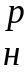
\includegraphics[width=0.8\textwidth]{assets/67}
% 	\caption*{}
% \end{figure},
% ккал/кг
% \end{minipage}} &
% \multirow{2}{=}{\begin{minipage}[b]{\linewidth}\raggedright
% Тепловой баланс ккал/кг
% \end{minipage}} \\
% & & \begin{minipage}[b]{\linewidth}\raggedright
% на аналитическую массу
% \end{minipage} & \begin{minipage}[b]{\linewidth}\raggedright
% на
% 
% сухую
% 
% массу
% \end{minipage} \\
% \midrule\noalign{}
% \endhead
% \bottomrule\noalign{}
% \endlastfoot
% 1 & Уголь исходный & - & 100 & 5752,81 & 5752,81 \\
% \multicolumn{6}{@{}>{\raggedright\arraybackslash}p{(\columnwidth - 10\tabcolsep) * \real{1.0000} + 10\tabcolsep}@{}}{%
% Продукты пиролиза угля} \\
% 1 & Полукокс & 84,76 & 88,29 & 5587,19 & 4735,70 \\
% 2 & Смола & 5,13 & 5,34 & 8745,14 & 448,62 \\
% 3 & Пирогенетическая вода & 2,39 & 2,49 & - & - \\
% 4 & Вода внешняя & 4,0 & - & - & - \\
% 5 & Газ & 3,72 & 3,87 & 7731,95 & 287,63 \\
% \multicolumn{2}{@{}>{\raggedright\arraybackslash}p{(\columnwidth - 10\tabcolsep) * \real{0.3390} + 2\tabcolsep}}{%
% Итого} & 100 & 100 & - & 5471,95 \\
% \multicolumn{4}{@{}>{\raggedright\arraybackslash}p{(\columnwidth - 10\tabcolsep) * \real{0.7226} + 6\tabcolsep}}{%
% Невязка баланса} & & 280,86
% 
% (4,88\%) \\
% \end{longtable}

\begin{multicols}{2}
Как видно из таблицы 10, невязка теплового баланса составляет менее 5 \%
(4,88 \%), что вполне допустимо и удовлетворяет требованиям по пределам
допустимой случайной погрешности невязки.

{\bfseries Выводы.} Проведенное исследование процесса низкотемпературного
пиролиза угля месторождения «Сарыадыр» показало, что основными
продуктами пиролиза являются полукокс (84,76 \%) и в небольших
количествах ̶ горючий газ (3,72 \%) и смола (5,13 \%). Полукокс
представляет собой высококачественное малосернистое твердое топливо.
Полученный полукокс характеризуется низким выходом летучих (10,81 \%) и
высокой теплотворной способностью (Qp= 5587,19 ккал/кг) и такой продукт может использован в качестве
эффективного бездымного топлива, а также в качестве восстановителя для
металлургической промышленности. Получаемый из угля горючий газ также
обладает высокой калорийностью. Таким образом, полученные из угля ценные
химические продукты могут быть эффективно использованы в области
энергетики.

\emph{{\bfseries Финансирование.} работа выполнена при финансовой поддержке
Комитета науки Министерства науки и высшего образования Республики
Казахстан (№ BR21882171 «ЦУР 9.4: Развитие «зеленой» экономики
Казахстана путем переработки минерального сырья и отходов методом
пиролиза»).}
\end{multicols}

\begin{center}
{\bfseries Литература}
\end{center}

\begin{noparindent}
1. Михайлова Е.С., Исмагилов 3.Р., Шикина Н.В. Исследование
физико-химических свойств катализаторов в реакции озонолиза
каменноугольного сырого бензола//Химия в интересах устойчивого
развития.- 2016.-Т.24(3).- С.369-377. DOI~10.15372/KhUR20160312

2. Кузнецов П.Н., Маракушина Е.Н., Бурюкин Ф.А., Исмагилов 3.Р.
Получение альтернативных пеков из углей // Химия в интересах устойчивого
развити.- 2016.-Т.24.(3)- С. 325-333. DOI 10.15372/KhUR20160307

3. Жеребцов С.И., Малышенко Н.В., Смотрина О.В., Брюховецкая Л.В.,
Исмагилов 3.Р. Сорбция катионов меди нативными и модифицированными
гуминовыми кислотами // Химия в интересах устойчивого развития.-
2016.-Т.24(3)- С.399 - 403.

DOI 10.15372/KhUR20160316

4. C.~Ma,~Y.~Zhao,~T.~Lang,~C.~Zou,~J.~Zhao,~Z.~Miao. Pyrolysis
characteristics of low-rank coal in a low-nitrogen pyrolysis atmosphere
and properties of the prepared chars// Energy.-2023.-~277(4): 127524.
DOI:10.1016/j.energy.2023.127524

5. P.R.~Solomon,~M.A.~Serio,~E.M.~Suuberg. Coal pyrolysis: experiments,
kinetic rates and mechanisms // Progress in Energy and Combustion
Science/-1992.-Vol.18~(2).- P.~133-220.

DOI 10.1016/0360-1285(92)90021-R

6. M.J.~Fabianska\emph{~}et al. Biomarkers, aromatic hydrocarbons and
polar compounds in the neogene lignites and gangue sediments of the
Konin and Turoszow Brown coal basins (Poland) // International Journal
of Coal Geology.-2013.-Vol 107.-P.24-44. DOI 10.1016/j.coal.2012.11.008.

7. M.X.~Liu\emph{~}et al. The radical and bond cleavage behaviors of 14
coals during pyrolysis with 9,10-dihydrophenanthrene // Fuel.-
2016.-182.- P. 480-486. DOI10.1016/j.fuel.2016.06.006.

8. M.~Baysal\emph{~}et al. Structure of some western Anatolia coals
investigated by FTIR, Raman,~\textsuperscript{13}C solid state NMR
spectroscopy and X-ray diffraction // International Journal of Coal
Geology.- 2016.-Vol. 163(1).- P.-166-176. DOI
10.1016/j.coal.2016.07.009.

9.Шантарин В.Д. Безальтернативный метод утилизации углеродсодержащих
отходов // Наука и Мир. 2014. № 9 (13). С. 41-45.

10. Исламов С.Р., Степанов С.Г. Глубокая переработка угля: введение в
проблему выбора технологии // Уголь.- 2007. - № 10 (978).- С. 53--58.

11. Y.~Liu,~Q.~Yao,~M.~Sun,~X.~Ma. Catalytic fast pyrolysis of coal tar
asphaltene over zeolite catalysts to produce high-grade coal tar: an
analytical Py-GC/MS study // Journal of Analytical and Applied
Pyrolysis.-2021.-156:~105127. DOI 10.1016/j.jaap.2021.105127

12. Y.~Che,~K.~Shi,~Z.~Cui,~H.~Liu,~Q.~Wang,~W.~Zhu,~et al. Conversion
of low temperature coal tar into high value-added chemicals based on the
coupling process of fast pyrolysis and catalytic cracking//
Energy.-2023.-~264:126169. DOI 10.1016/j.energy.2022.126169

13. Z.-H.~Ma,~X.-Y.~Wei,~G.-H.~Liu,~F.-J.~Liu,~Z.-M.~Zong. Value-added
utilization of high-temperature coal tar: a review.//
Fuel.-2021.-Vol.292:119954. DOI 10.1016/j.fuel.2020.119954

14. B.Purevsuren, S.Batbileg, M.Battsetseg, S.Jargalmaa, B.Avid,
A.Ariunaa, P.N.Kuznetsov, E.S. Kamenskii, L.I. Kuznetsova. Properties of
Mongolian Coal and Its Semicoking Products// Coke and
Chemistry.-2021.-Vol. 64(2).-P.58 - 63. DOI 10.3103/S1068364X21020058
\end{noparindent}

\begin{center}
{\bfseries References}
\end{center}

\begin{noparindent}
1. Mihajlova E.S., Ismagilov 3.R., Shikina N.V. Issledovanie
fiziko-himicheskih svojstv katalizatorov v reakcii ozonoliza
kamennougol\textquotesingle nogo syrogo benzola//Himija v interesah
ustojchivogo razvitija.- 2016.-T.24(3).- S.369-377. DOI
10.15372/KhUR20160312

{[}in Russ.{]}

2. Kuznecov P.N., Marakushina E.N., Burjukin F.A., Ismagilov 3.R.
Poluchenie al\textquotesingle ternativnyh pekov iz uglej // Himija v
interesah ustojchivogo razviti.- 2016.-T.24.(3)- S. 325-333. DOI
10.15372/KhUR20160307. {[}in Russ.{]}

3. Zherebcov S.I., Malyshenko N.V., Smotrina O.V., Brjuhoveckaja L.V.,
Ismagilov 3.R. Sorbcija kationov medi nativnymi i modificirovannymi
guminovymi kislotami // Himija v interesah ustojchivogo razvitija.-
2016.-T.24(3)- S.399 - 403. DOI 10.15372/KhUR20160316. {[}in Russ.{]}

4. C.~Ma,~Y.~Zhao,~T.~Lang,~C.~Zou,~J.~Zhao,~Z.~Miao. Pyrolysis
characteristics of low-rank coal in a low-nitrogen pyrolysis atmosphere
and properties of the prepared chars// Energy.-2023.-~277(4): 127524.
DOI:10.1016/j.energy.2023.127524

5. P.R.~Solomon,~M.A.~Serio,~E.M.~Suuberg. Coal pyrolysis: experiments,
kinetic rates and mechanisms // Progress in Energy and Combustion
Science/-1992.-Vol.18~(2).- P.~133-220.

DOI 10.1016/0360-1285(92)90021-R

6. M.J.~Fabianska\emph{~}et al. Biomarkers, aromatic hydrocarbons and
polar compounds in the neogene lignites and gangue sediments of the
Konin and Turoszow Brown coal basins (Poland) // International Journal
of Coal Geology.-2013.-Vol 107.-P.24-44. DOI 10.1016/j.coal.2012.11.008.

7. M.X.~Liu\emph{~}et al. The radical and bond cleavage behaviors of 14
coals during pyrolysis with 9,10-dihydrophenanthrene // Fuel.-
2016.-182.- P. 480-486. DOI10.1016/j.fuel.2016.06.006.

8. M.~Baysal\emph{~}et al. Structure of some western Anatolia coals
investigated by FTIR, Raman,~\textsuperscript{13}C solid state NMR
spectroscopy and X-ray diffraction // International Journal of Coal
Geology.- 2016.-Vol. 163(1).- P.-166-176. DOI
10.1016/j.coal.2016.07.009.

9.Shantarin V.D. Bezal\textquotesingle ternativnyj metod utilizacii
uglerodsoderzhashhih othodov // Nauka i Mir. 2014. № 9 (13). S. 41-45.
{[}in Russ.{]}

10. Islamov S.R., Stepanov S.G. Glubokaja pererabotka uglja: vvedenie v
problemu vybora tehnologii // Ugol\textquotesingle.- 2007. - № 10
(978).- S. 53--58. {[}in Russ.{]}

11. Y.~Liu,~Q.~Yao,~M.~Sun,~X.~Ma. Catalytic fast pyrolysis of coal tar
asphaltene over zeolite catalysts to produce high-grade coal tar: an
analytical Py-GC/MS study // Journal of Analytical and Applied
Pyrolysis.-2021.-156:~105127. DOI 10.1016/j.jaap.2021.105127

12. Y.~Che,~K.~Shi,~Z.~Cui,~H.~Liu,~Q.~Wang,~W.~Zhu,~et al. Conversion
of low temperature coal tar into high value-added chemicals based on the
coupling process of fast pyrolysis and catalytic cracking//
Energy.-2023.-~264:126169. DOI 10.1016/j.energy.2022.126169

13. Z.-H.~Ma,~X.-Y.~Wei,~G.-H.~Liu,~F.-J.~Liu,~Z.-M.~Zong. Value-added
utilization of high-temperature coal tar: a review.//
Fuel.-2021.-Vol.292:119954. DOI 10.1016/j.fuel.2020.119954

14. B.Purevsuren, S.Batbileg, M.Battsetseg, S.Jargalmaa, B.Avid,
A.Ariunaa, P.N.Kuznetsov, E.S. Kamenskii, L.I. Kuznetsova. Properties of
Mongolian Coal and Its Semicoking Products// Coke and
Chemistry.-2021.-Vol. 64(2).-P.58 - 63. DOI 10.3103/S1068364X21020058

\emph{{\bfseries Сведения об авторах}}

Нургалиев Н.У.-кандидат химических наук, ассоциированный профессор,
Казахский университет технологии и бизнеса имени К. Кулажанова, Астана
Казахстан, e-mail: nurgaliev\_nao@mail.ru;

Искакова Ж.Б.-кандидат химических наук, ассоциированный профессор,
Научно-исследовательский институт Новых химических технологий,
Евразийский национальный университет им. Л.Н. Гумилева,
Астана,Казахстан, e-mail: zhanariskakova@mail.ru;

Колпек А.-кандидат химических наук, ассоциированный профессор,
Евразийский национальный университет им. Л.Н. Гумилева, Астана,
Казахстан, e-mail: aynagulk@mail.ru;

Айбульдинов Е.Е. - доктор PhD, Научно-исследовательский институт Новых
химических технологий, Евразийский национальный университет им. Л.Н.
Гумилева, Астана, Казахстан, Астана, e-mail: elaman\_@mail.ru;

Сабитов А.С.-докторант, Евразийский национальный университет им. Л.Н.
Гумилева, Астана, Казахстан, e-mail: sawy552@gmail.com;

Копишев Э.К.-кандидат химических наук, Евразийский национальный
университет им. Л.Н. Гумилева, Астана, Казахстан, e-mail:
eldar\_kopishev@mail.ru;

Салихов Р.М.-главный инженер, ООО «ТТУ ЛТД», Российская Федерация, г.
Санкт-Петербург, e-mail: info.galotar@gmail.com;

Петров М.С.-главный инженер, ООО «ТТУ ЛТД», Российская Федерация, г.
Санкт-Петербург, e-mail: info.galotar@gmail.com;

Алжанова Г.Ж.- докторант,Евразийский национальный университет им. Л.Н.
Гумилева, Астана, Казахстан,e-mail: galiya.alzhanova@gmail.com;

Абдиюсупов Г.Г.-менеджер, ТОО «CCS Services - Central Asia», Астана,
Казахстан, e-mail: gaziz\_86@inbox.ru;

Өмірзақ М.Т.-доктор PhD, ТОО «Sauda Exports\&Import»,
Астана,Казахстан,e-mail: madi.omirzak@gmail.com
\end{noparindent}

\emph{{\bfseries Information about the authors}}

\begin{noparindent}
Nurgaliyev N.U.-Candidate of Chemical Science, Associate Professor,
Kazakh University of Technology and Business, Astana, Kazakhstan,
e-mail: nurgaliev\_nao@mail.ru;

Iskakova Zh.B.-Candidate of Chemistry Sciences, Associate Professor,
Research Institute of New Chemical Technologies, L.N. Gumilyov Eurasian
National University, Astana, Kazakhstan, e-mail: zhanariskakova@mail.ru;

Kolpek A.-Candidate of Chemistry Sciences, Associate Professor, L.N.
Gumilyov Eurasian National University, Astana, Kazakhstan, e-mail:
aynagulk@mail.ru;

Aybuldinov E.K.-PhD, Research Institute of New Chemical Technologies,
L.N. Gumilyov Eurasian National University, Astana, Kazakhstan, e-mail:
elaman\_@mail.ru;

Sabitov A.S.-Doctoral Student, L.N. Gumilyov Eurasian National
University, Astana, Kazakhstan, e-mail: sawy552@gmail.com;

Kopishev E.Ye.- Candidate of Chemistry Sciences, L.N. Gumilyov Eurasian
National University, Astana, Kazakhstan, e-mail:
eldar\_kopishev@mail.ru;

Salikhov R.M.-Chief Engineer, LLC "TTU LTD", Russian Federation, St.
Petersburg, e-mail: info.galotar@gmail.com;

Petrov M.S.-Chief Engineer, LLC "TTU LTD", Russian Federation, St.
Petersburg, e-mail: info.galotar@gmail.com

Alzhanova G. Zh.-Doctoral Student, Research Institute of New Chemical
Technologies, L.N. Gumilyov Eurasian National University, Astana,
Kazakhstan, e-mail: galiya.alzhanova@gmail.com;

Abdiyus{\bfseries s}upov G.G.-Manager, CCS Services -- Central Asia LLP,
Astana, Kazakhstan, e-mail: gaziz\_86@inbox.ru;

Ómirzak M.T.-PhD, Sauda Exports\&Import LLP, Astana, Kazakhstan, e-mail:
madi.omirzak@gmail.com
\end{noparindent}
